% The topic, motivation, the importance of adaptivity 



Consider a dataset $X$ consisting of $n$ independent samples from some unknown population $\dist$.  How can we ensure that the conclusions drawn from $X$ \emph{generalizes} to the population $\dist$?  Despite decades of research in statistics and machine learning on methods for ensuring generalization, there is an increased recognition that many scientific findings generalize poorly (e.g. 
\cite{Ioannidis05,GelmanL13}
).  While there are many reasons a conclusion might fail to generalize, one that is receiving increasing attention is \emph{adaptivity}, which occurs when the choice of method for analyzing the dataset depends on previous interactions with the same dataset~\cite{GelmanL13}.

 Adaptivity can arise from many common practices, such as exploratory data analysis, using the same data set for feature selection and regression, and the re-use of datasets across research projects.  Unfortunately, adaptivity invalidates traditional methods for ensuring generalization and statistical validity, which assume that the method is selected independently of the data. The misinterpretation of adaptively selected results has even been blamed for a ``statistical crisis'' in empirical science~\cite{GelmanL13}.
%  ~\cite{GelmanL13}.

\begin{figure}
    \centering
    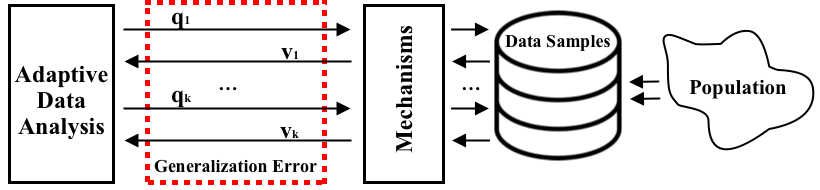
\includegraphics[width=0.7\columnwidth]{overview.png}
    \caption{Overview of our Adaptive Data Analysis model. We have a population that we are interested in studying, and a dataset containing individual samples from this population. The adaptive data analysis we are interested in running has access to the dataset through queries of some pre-determined family (e.g., statistical or linear queries) mediated by a mechanism. This mechanism uses randomization to reduce the generalization error of the queries issued to the data.}
    \label{fig:adaptivity-model-overview}
\vspace{-0.5cm}
\end{figure}

A line of work initiated by \citet{DworkFHPRR15}, \citet{HardtU14} posed the question: Can we design \emph{general-purpose} methods that ensure generalization in the presence of adaptivity, together with guarantees on their accuracy?  The idea that has emerged in these works is to use randomization to help ensure generalization. Specifically, these works have proposed to mediate the access of an adaptive data analysis to the data by means of queries from some pre-determined family (we will consider here statistical or linear queries) that are sent to a  \emph{mechanism} which uses some randomized process to guarantee that the result of the query does not depend too much on the specific
sampled dataset. This guarantees that the result of the queries generalizes well. This approach is described in Figure~\ref{fig:adaptivity-model-overview}.  
This line of work has identified many new algorithmic techniques for ensuring generalization in adaptive data analysis, leading to algorithms with greater statistical power than all previous approaches. Common methods proposed by these works include, the addition of noise to the result of a query, data splitting, etc. Moreover, these works have also identified problematic strategies for adaptive analysis, showing limitations on the statistical power one can hope to achieve. Subsequent works have then further extended the methods and techniques in this approach and further extended the theoretical underpinning of this approach, e.g.~\cite{dwork2015reusable,dwork2015generalization,BassilyNSSSU16,UllmanSNSS18,FeldmanS17,jung2019new,SteinkeZ20,RogersRSSTW20}.
%

A key development in this line of work is that the best method for ensuring generalization in an adaptive data analysis depends to a large extent on the number of \emph{rounds of adaptivity}, the depth of the chain of queries. As an informal example, the program $x \leftarrow q_1(D);y \leftarrow q_2(D,x);z \leftarrow q_3(D,y)$ has three rounds of adaptivity, since $q_2$  depends on $D$ not only directly because it is one of its input but also via the result of $q_1$, which is also run on $D$, and similarly,  $q_3$ depends on $D$ directly but also via the result of $q_2$, which in turn depends on the result of $q_1$. The works we discussed above showed that, not only does the analysis of the generalization error depend on the number of rounds, but knowing the number of rounds actually allows one to choose methods that lead to the smallest possible generalization error. As an example, when a study includes queries with a large number of rounds of adaptivity, then a low generalization error can be achieved by adding Gaussian noise scaled to the number of rounds to the result of each query.
When instead a study includes queries with a low number of rounds of adaptivity, then a low generalization error can be achieved by using more specialized methods, such as the reusable holdout technique from~\citet{DworkFHPRR15}. 




%gap
This scenario motivates us to explore the design of program analysis techniques that can be used to estimate the number of \emph{rounds of adaptivity} that a program implementing a data analysis can perform. These techniques could be ultimately be integrated into a tool for adaptive data analysis such as the \emph{Guess and Check} framework by~\citet{RogersRSSTW20}. 
%

The first problem we face is \emph{how to define formally} a model for adaptive data analysis which is general enough to support the methods we discussed above and would permit to formulate the notion of adaptivity these methods use. We take the approach of designing a programming framework for submitting queries to some \emph{mechanism} giving access to the data mediated by one of the techniques we mentioned before, e.g., adding Gaussian noise, randomly selecting a subset of the data, using the reusable holdout technique, etc. In this approach, a program models an \emph{analyst} asking a sequence of queries to the mechanism. The mechanism runs the queries on the data applying one of the methods discussed above and returns the result to the program. The program can then use this result to decide which query to run next. Overall, we are interested in controlling the generalization of the results of the queries which are returned by the mechanism, by means of the adaptivity. 

To define adaptivity we consider a dependency graph between the different queries that we synthesize from the possible execution traces of the program representing the data analysis. The dependency graph is built by inspecting all the possible traces of execution and by identifying situations where the execution of a query \emph{causes} the execution of another query. Intuitively, a query $Q$ may depend on another query $P$, if there are two values that $P$ can return which affect in different ways the execution of $Q$. 
For example, as depicted in \cite{dwork2015reusable}, a machine learning algorithm for constructing a classifier can be modeled by first computing each feature's correlations with the label via a sequence of queries, and then constructing the classifier based on the correlation values. If one feature's correlation changes, the classifier depending on features is also affected.  
This notion of dependency builds on the execution trace as a \emph{causal history}. In particular, we are interested in the history or provenance of a query up until this is executed, we are not then concerned about how the result is used --- except for tracking whether the result of the query may further cause some other query. This is because we focus on the generalization error of queries and not their post-processing.  

The second problem we face is \emph{how to estimate the adaptivity of a given program}. The adaptive data analysis model we consider and our definition of adaptivity suggest that for this task we can use a  program analysis that is reminiscent of information flow control. However, this is not sufficient since, in general, a query $Q$ is not a monolithic block but rather it may depend, through the use of variables and values, on other parts of the program. Hence, we also need to consider some form of data-flow analysis. Our program analysis, named {\THESYSTEM}, combines information flow and data-flow analysis using an adjacency matrix $M$ representing the dependency between different variables, and a vector $V$ representing different queries. These two components allow us to over-approximate the dependency graph and estimate the adaptivity of the program. 

To simplify our analysis, we do not directly apply the program analysis to the source program. Instead, we first transform the program into static single assignment form, SSA form. In this form all the variables are assigned once, including variables in loops, and this helps our analysis in avoiding the complexity of handling variables reassignment. Moreover, we show that by analyzing programs in SSA form, we get a bound on the number of rounds of adaptivity that is also a bound for the source program.


% \wq{According to the aforementioned work for ensuring generalization in adaptive data analysis, the tight generalization error bound is achieved under the analyst-mechanism assumption that, the analyzed program is modelled as a procedure of an \emph{analyst} asking a sequence of queries to some mechanism and only the responded answers are back to the {analyst}, with no processing of the query results revealed. Then The adaptivtity notion under this assumption, only focusing on the queries, is the length of a sequence of adaptively chosen queries among the queries asked by the {analyst}.}
% This requires us to define  Since most of these techniques we focus in this work on queries that can be executed \emph{row-by-row}, those submitted 
% queries are specified by some function of a row in the framework.
% and how to integrate the techniques mentioned before in a programming . Hence, as a first step we Nevertheless, the corresponding study on static analysis over programs implementing adaptive analysis is not well explored, even the formal definition of this \emph{rounds of adaptivity} is not clear. Our goal is to study adaptivity and conduct analysis over programs to find the number of rounds.
% our innovation

% Based on this framework, we define adaptivity as a property based on multiple traces of executions, or in other terms as an hyperproperty~\cite{clarkson2010hyperproperties}. \wq{For the sequence of adaptively chosen queries described before, the concept of one query may depend on its previous queries and answers is necessary. } Intuitively, a query $Q$ may depend on another query $P$, if there are two 
% values that $P$ can return which affect in different ways the execution of $Q$. 
% This definition suggests that we need to consider a program analysis which is a reminiscence of information flow control. However, this is not sufficient since, in general, a query is not a monolithic block $Q$ but rather some syntactic construction depending on some expression that depends on some variables. Hence, we also need to consider some data-flow analysis. 
% In a word, what we want is a program analysis which statically provides an upper bound on the number of rounds of adaptivity, and on the number of queries that are run by programs implementing adaptive data analysis. 

% The first question we need to decide on is what language the target programs to be analyzed are written, in a functional programming language or an imperative one?     
% the reason we do not use functional programming language, 
 %We choose the imperative programming language, then the following question is what does this imperative language look like? 
%  A principle of the ideal language in our mind is supposed to be simple enough to alleviate the burden of analysis on complex components that is unnecessary to adpativity, and expressive enough to support most of the adaptive data analysis algorithms. With this principle in mind, we introduce an imperative language called the {\tt Loop} language, with one finite loop construct, allowing data analysts recursively request queries in their programs. The query request is also supported in the language.

% The query request is abstract in the loop language and shows up as a primitive construct $q(e)$, where the argument $e$ is an expression tracking the necessary information needed to construct the unique query. We choose to make query abstract for the reason that we only care about the elements(the arguments) used to construct the query instead the detail of the query, with respect to what we are interested in: whether some queries rely on some other queries.        

%  For the number of rounds of adaptivity of program in the loop language, a definition of "one query relies on another query", or "one query may depend on the other" is the next big thing. We choose to define this "may-dependency" with the help of a trace-based operational semantics.  
% %  the change of the results of the query will affect the appearance of the other in a trace of the execution. The trace is
%  The trace is a list of queries generated along with the execution of the program, a history of the execution only caring about query requests.
%  which is specified in the operational semantics and will be discussed later.


% one is the transformation of programs of the aforementioned loop language we call it "high level language", to its variant "low level language", in which the arguments of queries go into the control flow of the program. Performing such a transformation helps us to better focus on the dependency between queries because we can treat queries simply as primitive symbols in the low level loop language without worrying about the arguments of the queries affecting the results. 
% In a word, the key idea of this transformation guarantees all the effect on queries comes from the structure of the programs. 
% The other is the transformation from the "low level" programs
% to construct a dependency graph between these unique variables, and hence predict the rounds of adaptivity from the graph. To generate the dependency graph, 
% To be more specific, our framework is equipped with algorithms to record the necessary information and construct a dependency graph to reach a final estimation of the adaptivity.

To Summarize, our work aims at the design of a static analysis for programs implementing adaptive analysis that can estimate their rounds of adaptivity. Specifically, our contributions are as follows:
\begin{enumerate}
    \item A programming framework for adaptive data analyses where the program represents an analyst that can query a generalization-preserving mechanism mediating the access to some data. 
    % \item A trace-based operational semantics for the loop language, specific to dependency between queries.
    \item A formal definition of the notion of adaptivity under the analyst-mechanism model. This definition is built on a query-based dependency graph built out of all the possible program execution traces.
    % \item A transformation between the {\tt Loop} language and the ssa language, with the soundness of the transformation.
    \item A program analysis algorithm {\THESYSTEM} which provides an upper bound on the adaptivity via a variable-based dependency graph.
    \item A soundness proof of the program analysis showing that the adaptivity estimated by {\THESYSTEM} bounds the true adaptivity of the program. 
\end{enumerate}



